%
\documentclass[11pt]{book}
%\pagestyle{plain}
\usepackage{makeidx}
%\usepackage{graphicx}

\usepackage{multirow} % Needed for cells in tables that span rows
\usepackage{listings} % for \lstset , listing code (chptr-code-listing)
\usepackage{color}   % make code pretty
\usepackage{multicol} % for a multi-column list
\usepackage{hyperref} % for \url , \href , etc.
\usepackage{framed} % for \framed
%\usepackage{pdfpages} % for \includepdf

%?? - Huh?  Can't get \k{} sequence
%\usepackage[T1]{fontenc}
%\usepackage[utf8]{inputenc}

%------- lstsetlisting settings  -------------

\definecolor{dkgreen}{rgb}{0,0.6,0}
\definecolor{gray}{rgb}{0.5,0.5,0.5}
\definecolor{dkred}{rgb}{0.8, 0, 0}
\definecolor{seablue}{rgb}{0, 0.5, 1}

\lstset{%
  basicstyle={\small\ttfamily},
	frame=single,
  language=C,
  aboveskip=3mm,
  belowskip=3mm,
  showstringspaces=false,
  columns=flexible,
  numbers=none,
  numberstyle=\tiny\color{blue},
	%identifierstyle=\color{seablue},
  keywordstyle=\color{dkgreen},
  commentstyle=\color{gray},
  stringstyle=\color{dkred},
  breaklines=false,
	resetmargins=true,
  %breakatwhitespace=true,
  tabsize=3
}


%%%%%%  Top Matter  %%%%%%%%%%%%%%%
\title{First Book}
\author{Kurt Schmidt}
\date{Aug 2014}

\begin{document}

\maketitle % ?? Use this for books?

%%%%%%  Front Matter  %%%%%%%%%%%%%%%
\frontmatter
\tableofcontents

%%%%%%  Main Matter  %%%%%%%%%%%%%%%
\mainmatter

\chapter{In a Galaxy, Far Far Away}
\label{starwars} % So I can \ref{altrings} later.

\section{Notes}
\label{notes}
%\input{chap1/sec11}

I'm just working my way through \LaTeX.  I put some Latex code here, and as
I gain proficiency, perhaps I'll put more.  For now, it would be helpful to
look at the source, as you read the book.  They should be in the same
directory.

Note, if the margins look odd on alternate pages, this is a \texttt{book}
document, meant to be bound.

For a text, this style of paragraph indentation/spacing is not so ideal.
I'll play later, but, for now, try playing with \texttt{
\textbackslash{}setlength\{\textbackslash{}parindent\}[\textit{width}] } and
\texttt{
\textbackslash{}setlength\{\textbackslash{}parskip\}[\textit{width}] }

Read up on \emph{rubber lengths}.  Also, be careful using \texttt{parskip}, as
it affects spacing in lists and other places.  The \texttt{parskip} package
might be helpful here.

\section{Heather Graham}
\label{graham}
%\input{chap1/sec12}
Talented, lovely.  And just gets more so.

\section{Compiling}

There should be a makefile in this directory, but I'm not at all happy with
it.

Also, I'm having issues using CYGWIN\_NT\-6.1 XXXXX 1.7.9(0.237/5/3)
2011-03-29 10:10 i686 Cygwin.  Packages are missing, compilation is somehow
more painful.  But, it's a pretty old install, so.  Ah, versions:

\begin{verbatim}
	$ latex --version
	pdfeTeX 3.141592-1.21a-2.2 (Web2C 7.5.4)
	kpathsea version 3.5.4
\end{verbatim}

Oh, did ya catch some approximation of $\pi$ in there?

On tux, we have:

\begin{verbatim}
	$ latex --version
	pdfTeX 3.1415926-1.40.10-2.2 (TeX Live 2009/Debian)
	kpathsea version 5.0.0
\end{verbatim}

Much newer version, anyway.  I should maybe update this thing.

Anyway, two ways I've been compiling TEX to PDF.  The first is two steps,
TEX$\rightarrow$DVI, then DVI$\rightarrow$PDF:

\begin{verbatim}
	$ latex book.tex
	...
	$ dvipdf book.dvi
	...
\end{verbatim}

The second way accomplishes the task in a single step:

\begin{quote}
	\texttt{
		\$ pdflatex book.tex
		...
	}
\end{quote}

Hmmmm.  \texttt{pdflatex} isn't creating a table of contents for me on tux,
either.  Oh!  Run it a couple times in succession.  \texttt{bibtex} might be
in there somewhere.

Also, \texttt{pdflatex} will allow you to use PDF-specific commands, and
seems to be recommended.

Note, if using references, indices, table of contents, etc., pay attention
to the output.  A 2\textsuperscript{nd} run might be suggested.

\subsection{Compiler Warnings and Errors}

You'll see various informational warnings:

\begin{quote}
	\texttt{
		LaTeX Font Warning: Font shape `OMS/cmtt/m/n' undefined
		...
	}
\end{quote}

You want to make sure that a correct substitution was made, but these are
fairly harmless.

Errors, of course, need to be corrected, and will leave you at an
interactive prompt (until I figure out how to signal batchmode).  I find
\bf{\texttt{x}} or \bf{\texttt{q}} to be helpful.



\chapter{Basics}
\label{basics} 

Okay, I'm still working on my own understanding here, so, this is not etched
in stone.


\section{Hello, World}
\label{hello}

You knew it was coming.  You expected it.  You'd've been disappointed by its
absence.

%TODO  do this right, dammit

A basic \LaTeX document, article-style:

%TODO  Figure out how to get 80 columns to fit inside this box.  Smaller
% font?
\lstinputlisting[language=TeX,numbers=left]{hello.tex}

Until I get better, you're gonna want to grab the file yourself and compile
using \texttt{pdflatex} , see what the output looks like.

%\hline
%% hello.tex - simple example using the article
%
% 
\documentclass[a4paper,12pt,titlepage]{article}
\pagestyle{plain}
\title{Hello, World}
\author{Kurt Schmidt \\
	Drexel, Computer Science}
\date{Sept. 2014}

\begin{document}
\maketitle

Here's your obligatory `hello':  ``Hello.  Welcome to \LaTeX.''  \TeX is the
basic language, Developed by Donald Knuth.  \LaTeX is a way handy extension
to \TeX.  So, basic syntax probably applies to both.  Once we get into
packages, I've not clue, as yet, so, I'll just be talking about \LaTeX.

Easiest way to compile to PDF is using \texttt{pdflatex}.

\section{Math}
\label{hellomath}

And now, some math.  Remember, $\sum_{i=1}^m i = \frac{m(m+1)}{2}$, along
with identities for sums, and the sum of a geometric series.  You'll be
needing them.

Also recall these gems, you'll be needing them, too:

\[ b^{\log_{b}{x}} = x \]
\[ \log_{b}{b^x} = x \]
\[ \log_{b}{xy} = \log_{b}{x} + \log_{b}{y} \]
\[ \log_{b}{x/y} = \log_{b}{x} - \log_{b}{y} \]
\[ \log_{b}{x^n} = n\log_{b}{x} \]

So, 

\[ x^{\log_{b}{y}} = y^{\log_{b}{x}} \]

\section*{El Fin du Monde}
\label{end}

And that's it for now.  See section \ref{hellomath}.

\end{document}

%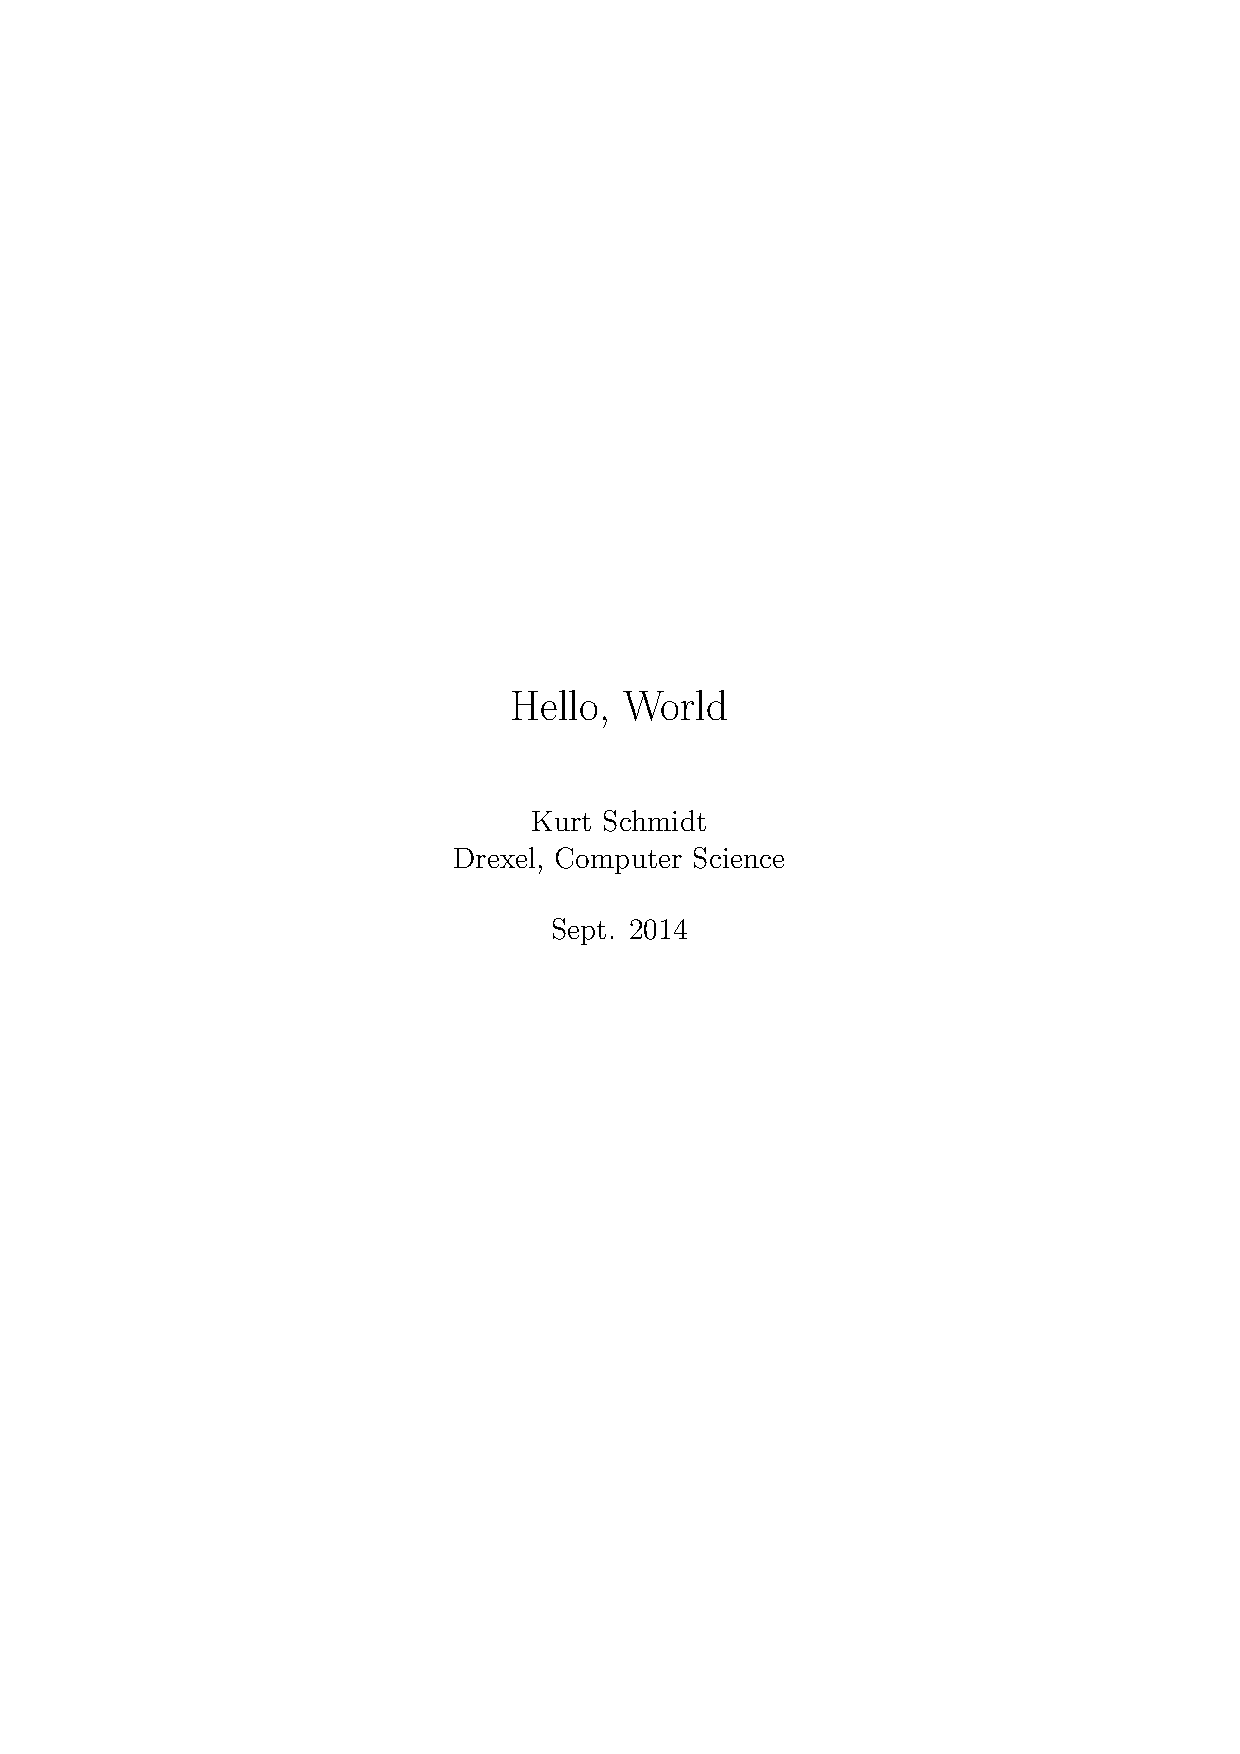
\includepdf{hello.pdf}

\section{Modes}
\label{modes-intro}

\TeX supports 2 basic modes, math and text.

When you're typing along, you're entering text.  Mostly you can just type as
you would, with a few exceptions.  There are metacharacters, paragraphs are
separated by two (or more) newlines.  We'll also want to talk about quotes,
hyphens and spaces.

Lines 24 and 30-34, in our hello example, show some uses of math mode.
See Section \ref{math} for a bit longer discussion.


\section{Metacharacters}
\label{metacharacters}

The following characters can not simply be typed, as they have special
meaning to \LaTeX{}:

\begin{quote}
	\{~~\}~~\$~~\%~~\_~~\&~~\#~~\^{}~~\textbackslash{}~~\~{}
\end{quote}

Here is how to print these characters in \LaTeX{}.  These metacharacters
will be explained, but for the moment, trust me.

\begin{center}
	\begin{tabular}{|c|l|}
		\hline
			\bf{Symbol} & \bf{\TeX sequence} \\
		\hline
			\{ & \textbackslash{}\{ \\
		\hline
			\} & \textbackslash{}\} \\
		\hline
			\$ & \textbackslash{}\$ \\
		\hline
			\% & \textbackslash{}\% \\
		\hline
			\& & \textbackslash{}\& \\
		\hline
			\# & \textbackslash{}\# \\
		\hline
			\_ & \textbackslash{}\_ \\
		\hline
			\textbackslash & \textbackslash{}textbackslash \\
		\hline
			\'{} & \textbackslash{}\'{}\{\} \\
		\hline
			\`{} & \textbackslash{}\`{}\{\} \\
		\hline
			\^{} & \textbackslash{}\^{}\{\} \\
		\hline
			\~{} & \textbackslash{}\~{}\{\} \\
			\textasciitilde & \textbackslash{}textasciitilde \\
			$\sim$ & \$\textbackslash{}sim\$ \\
		\hline
	\end{tabular}
\end{center}


\subsection{Braces for Grouping}

\{ \} are used for grouping.  Empty braces can be used to protect a special
symbol from immediate following text.  E.g.,
\texttt{\textbackslash{}textbackslash\{\}foo} would display
\textbackslash{}foo , since \texttt{\textbackslash{}textbackslashfoo} isn't
a character.


\subsection{Spaces}

Whitespace serves to separate words, etc, but in a typeset environment,
sequences of spaces, e.g., aren't of fixed size.

The \~{} in \LaTeX is a \emph{non-breaking space}.

If\textvisiblespace{}you\textvisiblespace{}want\textvisiblespace{}visible\textvisiblespace{}spaces,
use \textbackslash{}textvisiblespace\{\}.


\subsection{Quotes}
\label{basicquotes}

\LaTeX uses \`{}\`{} for left double quote, and \'{}\'{} for right double quote.
Similarly, \`{} and \'{} are used for left and right single quotes.

George said, `I heard an oldtimer once exclaim ``Oh, batshit!''{}'


\subsection{Dashes and Hyphens}

I believe the solitary \texttt{ - } is okay, though it might signal a
wordsplit, so, keep it in mind, if you have problems.  Well, let's see:
jack-in-the-box .

Two hyphens, \texttt{ -{}- }, yields an endash, --, and three, \texttt{
	-{}-{}- },  will give you an emdash, ---.

So, if you want 2 or more literal adjacent hyphens, -{}-, to keep the
sequence from being interpreted, use an empty string to separate them:
\texttt{ -\{\}-\{\}- } yields -{}-{}- .


\section{Special Characters}
\label{specchars}

Even if I knew what I was doing, this is a messy area.  For sanity's sake,
you want to restrict yourself to the 7-bit ASCII characters, and use \LaTeX
to create other characters.

You can change input encodings, \texttt{latin1}, \texttt{utf8}, etc., and
we're already past what I know.

We can represent many characters using escape codes.  Some special
characters are recognised in text mode, others only in math mode.

\subsection{Composition and Decoration}

We can add various accents and other decorations to any character.  Here are
a few:

%?? Is center the best environment for a table
\begin{center}
	\begin{tabular}{|l|c|}
		\hline
			\bf{Symbol} & \bf{\TeX sequence} \\
		\hline
		\texttt{ \textbackslash{}\`{}\{a\} } & \`{a} \\
		\texttt{ \textbackslash{}\'{}\{e\} } & \'{e} \\
		\texttt{ \textbackslash{}\"{}\{u\} } & \"{u} \\
		\texttt{ \textbackslash{}.\{o\} } & \.{o} \\
		\texttt{ \textbackslash{}\~{}\{n\} } & \~{n} \\
%		\texttt{ \textbackslash{}k\{a\} } & \k{a} \\  % KS - can't get the \k{}
%		sequence in OT1
		\hline
	\end{tabular}
\end{center}

Use \texttt{\textbackslash{}i} and \texttt{\textbackslash{}j} for the dotless
versions, so, \texttt{ \textbackslash{}\^{}\{\textbackslash{}i\} } to get \^{\i} .

Note, if you want a literal backtick, rather than a left single quote, you'd
be tempted to use \texttt{ \textbackslash{}\'{} }, but that is an esace
sequence for the grave accent, expecting a character to follow, so, give it
an empty string to act upon: \texttt{ \textbackslash{}\'{}\{\} }


\subsection{Other Defined Characters and Symbols}

Here's a quick list of some:

%?? TODO a multi-column table, in (newspaper) columns.

\begin{center}
	\begin{tabular}{|lc|}
		\hline
		\texttt{ \textbackslash{}l } & \l \\
		\texttt{ \textbackslash{}o } & \o \\
		\texttt{ \textbackslash{}TeX } & \TeX \\
		\texttt{ \textbackslash{}LaTeX } & \LaTeX \\
		\texttt{ \textbackslash{}textless } & \textless \\
		\texttt{ \textbackslash{}textgreater } & \textgreater \\
		\texttt{ \textbackslash{}S } & \S \\
		\texttt{ \textbackslash{}P } & \P \\
		\texttt{ \textbackslash{}dag } & \dag \\
		\texttt{ \textbackslash{}ddag } & \ddag \\
		\texttt{ \textbackslash{}copyright } & \copyright \\
		\hline
	\end{tabular}
\end{center}


\subsection{Common Symbols and Characters from Packages}

Okay, if it's a character, then it's available somewhere, often in several
flavors.  E.g., the official Euro sign, compared to one that'll display
nicely w/the currently selected font (bold, italic, etc.).

\begin{lstlisting}[language=Tex]
	\usepackage[gen]{eurosym}
\end{lstlisting}

will let you use \texttt{ \textbackslash{}euro\{\} }.

\begin{lstlisting}[language=Tex]
	\usepackage{textcomp}
\end{lstlisting}

will give you \texttt{ \$30\textbackslash{}textdegree angle\$ } (in math mode,
confusingly enough).

Or, for temperatures, you might instead

\begin{lstlisting}[language=Tex]
	\usepackage{gensymb}
\end{lstlisting}

, and use \texttt{ 21\textbackslash{}degree{}C }, or \texttt{
	21\textbackslash{}celsius }


\subsection{Math Symbols}
\label{intmathsymb}

Okay, in math mode you have access to many other symbols.  You'll see
examples of writing equations and such in Chapter \ref{math}. 

A few common symbols:

\begin{multicols}{2}
	\begin{tabular}{|l|c|}
		\hline
		\multicolumn{2}{|c|}{Relational Operators} \\
		\hline
		$=$ & = \\
		$\neq$ & \textbackslash{}neq \\
		$\equiv$ & \textbackslash{}equiv \\
		$\approx$ & \textbackslash{}approx \\
		$\sim$ & \textbackslash{}sim \\
		$\propto$ & \textbackslash{}propto \\
		$>$ & > \\
		$\gg$ & \textbackslash{}gg \\
		$\leq$ & \textbackslash{}leq \\
		$\succ$ & \textbackslash{}succ \\
		$\preceq$ & \textbackslash{}preceq \\
		$\subseteq$ & \textbackslash{}subseteq \\
		$\supset$ & \textbackslash{}supset \\
		$\in$ & \textbackslash{}in \\
		$\ni$ & \textbackslash{}ni \\
		$\cap$ & \textbackslash{}cap \\
		$\bigcup$ & \textbackslash{}bigcup \\
		$\vee$ & \textbackslash{}vee \\
		$\bigwedge$ & \textbackslash{}bigwedge \\
		$\parallel$ & \textbackslash{}parallel \\
		$\perp$ & \textbackslash{}perp \\
		\hline
	\end{tabular}
	\begin{tabular}{|l|c|}
			\hline
		\multicolumn{2}{|c|}{Binary Operators} \\
			\hline
		$\times$ & \textbackslash{}times \\
		$\div$ & \textbackslash{}div \\
		$\setminus$ & \textbackslash{}setminus \\
		$\cap$ & \textbackslash{}cap \\
		$\bigcup$ & \textbackslash{}bigcup \\
		$\bigwedge$ & \textbackslash{}bigwedge \\
		$\vee$ & \textbackslash{}vee \\
		$\oplus$ & \textbackslash{}oplus \\
		$\bigotimes$ & \textbackslash{}bigotimes \\
			\hline
	\end{tabular}
	\begin{tabular}{|l|c|}
			\hline
		\multicolumn{2}{|c|}{Other Set} \\
			\hline
		$\emptyset$ & \textbackslash{}emptyset \\
		$\infty$ & \textbackslash{}infty \\
			\hline
	\end{tabular}
	\begin{tabular}{|l|c|}
			\hline
		\multicolumn{2}{|c|}{Logic} \\
			\hline
		$\exists$ & \textbackslash{}exists \\
		$\exists!$ & \textbackslash{}exists! \\
		$\forall$ & \textbackslash{}forall \\
		$\neg$ & \textbackslash{}neg \\
		$\lor$ & \textbackslash{}lor \\
		$\land$ & \textbackslash{}land \\
		$\leftarrow$ & \textbackslash{}leftarrow \\
		$\iff$ & \textbackslash{}iff \\
			\hline
	\end{tabular}
	\begin{tabular}{|l|c|}
			\hline
		\multicolumn{2}{|c|}{Greek Letters} \\
			\hline
		$\Sigma$ & \textbackslash{}Sigma \\
		$\sigma$ & \textbackslash{}sigma \\
			\hline
	\end{tabular}
\end{multicols}

\begin{multicols}{2}
	\begin{tabular}{|l|c|}
			\hline
		\multicolumn{2}{|c|}{Other Arrows} \\
			\hline
		$\rightarrow$ & \textbackslash{}rightarrow \\
		$\Leftarrow$ & \textbackslash{}Leftarrow \\
		$\longrightarrow$ & \textbackslash{}longrightarrow \\
		$\uparrow$ & \textbackslash{}uparrow \\
		$\Downarrow$ & \textbackslash{}Downarrow \\
		$\updownarrow$ & \textbackslash{}updownarrow \\
			\hline
	\end{tabular}
	\begin{tabular}{|l|c|}
			\hline
		\multicolumn{2}{|c|}{Delimiters} \\
			\hline
		$[$ & \textbackslash{}[ \\
		$\langle$ & \textbackslash{}langle \\
		$\rceil$ & \textbackslash{}rceil \\
		$\lfloor$ & \textbackslash{}lfloor \\
			\hline
	\end{tabular}
	\begin{tabular}{|l|c|}
			\hline
		\multicolumn{2}{|c|}{Other Fun} \\
			\hline
		$\ldots$ & \textbackslash{}ldots \\
		$\cdots$ & \textbackslash{}cdots \\
		$\surd$ & \textbackslash{}surd \\
		$\flat$ & \textbackslash{}flat \\
		$\natural$ & \textbackslash{}natural \\
		$\sharp$ & \textbackslash{}sharp \\
		$\spadesuit$ & \textbackslash{}spadesuit \\
		$\heartsuit$ & \textbackslash{}heartsuit \\
		$\diamondsuit$ & \textbackslash{}diamondsuit \\
		$\clubsuit$ & \textbackslash{}clubsuit \\
			\hline
	\end{tabular}
\end{multicols}


There are others, and packages containing still more.

Functions and other mathematical constructs will be covered in Chapter
\ref{math}--Math Equations.


\chapter{Math}
\label{math} 

Placeholder.  I've not gotten here yet.



\chapter{Tables}
\label{tables} % So we can \ref{tables} later.

I took this mostly from http://www.andy-roberts.net/writing/latex/tables .

\section{Simple Tables}
\label{simple}

Introduce tables with the \emph{tabular} environment, describing columns.

\begin{quote}
	\texttt{ \textbackslash{}begin\{tabular\}\{ l c r \} }
\end{quote}

\begin{center}
	\begin{tabular}{ l r }
		l & left justified \\
		c & centered \\
		r & right justified \\
	\end{tabular}
\end{center}

\subsection{Vertical Lines}

Use the $\vert$ or $\Vert$ in the declaration for vertical separators.

\begin{center}
	\begin{tabular}{ l || r | }
		l & left justified \\
		c & centered \\
		r & right justified \\
	\end{tabular}
\end{center}

\subsection{Content of Tables}

Cells in a record are separated by \texttt{\&} .  
\textbackslash{}\textbackslash{} to start a new record.

Finally, use \texttt{\textbackslash{}hline} to put horizontal lines in:

\begin{center}
	\begin{tabular}{ l | r | }
		\hline 
		l & left justified \\
		\hline 
		c & centered \\
		\hline 
		r & right justified \\
		\hline 
	\end{tabular}
\end{center}


\section{Wrapping Text}
Sadly, \LaTeX doesn't wrap long lines in tables, by default.  It does
provide 3 other column specifiers which take a width argument, in
\texttt{pt}, \texttt{in}, \texttt{cm}, \texttt{mm}, or \texttt{em}:

\begin{center}
	\begin{tabular}{ | l | p{8cm} | }
		\hline
		Character & Meaning \\
		\hline
		\texttt{p\{$width$\}}
			& Paragraph column with text aligned vertically at the top \\
		\hline
		\texttt{m\{$width$\}}
			& Paragraph column with text vertically aligned in the middle (requires
			array package) \\
		\hline
		\texttt{b\{$width$\}}
			& Paragraph column with text vertically aligned at the bottom (requires
			array package) \\
		\hline
	\end{tabular}
\end{center}

The declaration for this table looks like:

\begin{quote}
	\texttt{ \textbackslash{}begin\{tabular\}\{ $\vert$ l $\vert$ p\{8cm\} $\vert$ \} }
\end{quote}

So, you'll need to play around a little, get it to come out nice.  Or, there
are packages already developed which'll do much of the work for you.

\section{Aligning on the Radix}
\label{radalign}

Again, there are packages that'll do this for you.  But, we're here, so...

\subsection{@-Expressions}
\label{atexpr}

Generally, the @ specifier takes a text argument, and a width specifier.
When appended to a column, it supresses normal cell spacing, and inserts the
text before each cell's contents.

We're going to use it without any space, to just use the radix to join two
columns of numbers (the integer and fractional parts).

\subsection{Tables of Numbers}

\begin{center}
	\begin{tabular}{ r @{.} l }
		123 & 456 \\
		3&14159265358979\\
		98765432 & 1 \\
	\end{tabular}
\end{center}


\section{Spanning}
\label{tablespan}

\subsection{Cell Spanning Multiple Columns}

In the data, place:

\begin{quote}
	\texttt{ \textbackslash{}multicolumn\{$numcols$\}\{$alignment$\}\{$contents$\} }
\end{quote}

, where $numcols$ is the number of subsequent columns (the width of this
cell, in columns), $alignment$ is one of \texttt{l}, \texttt{c}, or
\texttt{r} (maybe \texttt{p}?), with vertical separators, and, finally, the
contents of the cell.

\begin{center}
	\begin{tabular}{|r|l|}
		\hline
		\multicolumn{2}{|c|}{Endless Summer} \\
		\hline
		LOA & 43'5" \\
		\hline
		LWL & 36'4" \\
		\hline
		Beam & 12'10" \\
		\hline
		Draught & 5'11" \\
		\hline
		Displacement & 19,620 lbs \\
		\hline
		Fuel (diesel) & 63 gal \\
		\hline
		H$_2$O & 153 gal \\
		\hline
	\end{tabular}
\end{center}

\subsection{Cell Spanning Multiple Rows}

A cell spanning multiple rows is introduced with:

\begin{quote}
	\texttt{ \textbackslash{}multirow\{$numrows$\}\{$width$\}\{$contents$\} }
\end{quote}

To use this, you'll need the \texttt{multirow} package:

\begin{quote}
	\texttt{ \textbackslash{}usepackage\{multirow\} }
\end{quote}


, where $width$ could be a fixed width, or just use \* for the natural
width.

\begin{center}
	\begin{tabular}{|l|r|l|}
		\hline
		\multicolumn{3}{|c|}{Endless Summer} \\
		\hline
		\multirow{7}{*}{Specs}
			& LOA & 43'5" \\
			& LWL & 36'4" \\
			& Beam & 12'10" \\
			& Draught & 5'11" \\
			& Displacement & 19,620 lbs \\
			& Fuel (diesel) & 63 gal \\
			& H$_2$O & 153 gal \\
			\hline
		\multirow{5}{*}{Accomodations}
			& Cabins & 3 \\
			& Double Berths & 4 \\
			& Single Berths & 0 \\
			& Heads & 2 \\
			& Showers & 3 \\
			\hline
		\multirow{3}{*}{Rigging}
			& Masts & 1 \\
			\hline
			& \multicolumn{2}{|l|}{Furling main} \\
			& \multicolumn{2}{|l|}{Furling genoa} \\
			\hline
	\end{tabular}
\end{center}

Huh.  That \textbackslash{}hline went all the way through. I dunno.  Either
choose a package to help you make tables, or try embedding a table in the
table.

\section{Don't know yet}
\label{hold}

Whistling.


\chapter{Embedding Code in Text}
\label{embeddingcode} 

\section{Inlining Code in Text}
\label{inlinecode}

Use the  \texttt{ \textbackslash{}texttt\{\textit{code}\} } to inline a bit of code
in a paragraph.

You'll need to change text colors yourself.

\subsection{ Define Your Own Command }

You can define your own:

\begin{quote}
	\texttt{
		\textbackslash{}newcommand\{\textbackslash{}code\}[1]\{\textbackslash{}texttt\{\#1\}\}
	}
\end{quote}

\newcommand{\code}[1]{\texttt{#1}}

So you could then use the new command in-line 
\texttt{ \textbackslash{}code\{\textit{code}\} }

Honestly, not sure about this yet.  We'll get there.


\section{ Blocks of code }
\label{codeblock}

\subsection{ \texttt{verbatim} Environment }
\label{verbatim}

You can place a code block in a \texttt{verbatim} environment.  It seems that
all (most? many?) metacharacter behaviors are inhibited, and line breaks are
preserved.  I'm not so sure about leading white space.

\texttt{
	\textbackslash{}begin\{verbatim\}
		...
	\textbackslash{}end\{verbatim\}
}

Let's see how this looks:

\begin{verbatim}
   #include <stdio.h>

   char *name = "Kurt" ;

   int main( int argc, char *argv[] )
   {
      printf( "Hello, %s!\n", name ) ;

      return( 0 ) ;
   }  /* main */
\end{verbatim}

Hmmm.  Okay.  Moving on...


\subsection{ The \texttt{listings} Package }
\label{ listingspkg }

The \texttt{listings} package is part of \LaTeX{}'s standard library, I
believe.  It knows many languages (I hope), converts tabs to spaces you specify,
and, with the \texttt{color} package, will highlight literals, keywords,
comments, etc.  I do not yet know if you can define your own languages.

Here is an example, found on StackOverflow (see comment):

% This was ganked from
% http://stackoverflow.com/questions/3175105/how-to-insert-code-into-a-latex-doc

\begin{quote}
	\begin{verbatim}
   \usepackage{listings}
   \usepackage{color}

   \definecolor{dkgreen}{rgb}{0,0.6,0}
   \definecolor{gray}{rgb}{0.5,0.5,0.5}
   \definecolor{dkred}{rgb}{1, 0.6, 0.6}

   \lstset{frame=tb,
      language=C,
      aboveskip=3mm,
      belowskip=3mm,
      showstringspaces=false,
      columns=flexible,
      basicstyle={\small\ttfamily},
      numbers=none,
      numberstyle=\tiny\color{blue},
      keywordstyle=\color{dkgreen},
      commentstyle=\color{gray},
      stringstyle=\color{dkred},
      breaklines=true,
      breakatwhitespace=true,
      tabsize=3
   }
	\end{verbatim}
\end{quote}

You can, of course, define and use whichever colors you like.  Change default
language in the middle of document with
\texttt{\textbackslash{}lstset\{language=\textit{lang} \} } .

Then place your code in a \texttt{lstlisting} environment.  Let's see if we can
make our previous example better:


\begin{lstlisting}
	#include <stdio.h>

	char *name = "Kurt" ;

	int main( int argc, char *argv[] )
	{
		printf( "Hello, %s!\n", name ) ;

		return( 0 ) ;
	}  /* main */
\end{lstlisting}

You can even pull code right from a file, using

\begin{quote}
	\texttt{ \textbackslash{}lstinputlisting[language=Python]\{hello.py\} }
\end{quote}

%\lstset{language=Python}
%\lstinputlisting{hello.py}
\lstinputlisting[language=Python]{hello.py}

Nice.  Let's see if this is a better way to embed LaTeX.  There's a
\texttt{TeX} language listed.

\begin{lstlisting}[language=TeX]
You can even pull code right from a file, using \texttt{lstinputlisting}

	\lstinputlisting[language=Python]{hello.py}

So, I suppose this is for indented math expressions (note the super and
subscripts in math mode)

	\[ |f(y) - f(x)| < \epsilon \]
	\[ p_{i} = p_{i-1}^2 \]

\end{lstlisting}

Not exciting, but it works.


\subsection{Language Supported by \texttt{listings}}

This is according to \url{%
http://en.wikibooks.org/wiki/LaTeX/Source_Code_Listings#Supported_languages
} .  I don't see a date, know how current it is.

\begin{multicols}{4}
	\begin{itemize}
	\renewcommand{\labelitemi}{ }
		\item ABAP
		\item ACSL
		\item Ada
		\item Algol
		\item Ant
		\item Assembler
		\item Awk
		\item bash
		\item Basic
		\item C
		\item C++
		\item Caml
		\item Clean
		\item Cobol
		\item Comal
		\item csh
		\item Delphi
		\item Eiffel
		\item Elan
		\item erlang
		\item Euphoria
		\item Fortran
		\item GCL
		\item Gnuplot
		\item Haskell
		\item HTML
		\item IDL
		\item inform
		\item Java
		\item JVMIS
		\item ksh
		\item Lisp
		\item Logo
		\item make
		\item Mathematica
		\item Matlab
		\item Mercury
		\item MetaPost
		\item Miranda
		\item Mizar
		\item ML
		\item Modelica
		\item Modula-2
		\item MuPAD
		\item NASTRAN
		\item Oberon-2
		\item OCL
		\item Octave
		\item Oz
		\item Pascal
		\item Perl
		\item PHP
		\item Plasm
		\item PL/I
		\item POV
		\item Prolog
		\item Promela
		\item Python
		\item R
		\item Reduce
		\item Rexx
		\item RSL
		\item Ruby
		\item S
		\item SAS
		\item Scilab
		\item sh
		\item SHELXL
		\item Simula
		\item SQL
		\item tcl
		\item TeX
		\item VBScript
		\item Verilog
		\item VHDL
		\item VRML
		\item XML
		\item XSLT
	\end{itemize}
\end{multicols}

Take a peek at the link, above, there are notes I didn't bother with.
Various dialects of some of the languages are understood.

I was feelin' pretty good about the number of languages I'm familiar with,
'til I saw this list.  I've not even heard of some of these.



%%%%%%  Back Matter  %%%%%%%%%%%%%%%
\backmatter
%TODO get index working
\printindex  % Automagic?  Ah, needed the package.  Still doing nothing.
%bibliography.  TODO.  Not there yet

\end{document}
